\documentclass[a4paper, french, openany, 12pt]{book}
\usepackage[utf8]{inputenc}
\usepackage[T1]{fontenc}
\usepackage{babel}
\usepackage{pifont}
\usepackage{graphicx}
\usepackage{fullpage}
\usepackage[dvipsnames]{xcolor} % colors
\usepackage{tabto}
\usepackage{stackengine}
\usepackage[skip=20pt]{parskip} % space between paragraphs
\usepackage[hidelinks]{hyperref} % links
\usepackage[framemethod=TikZ]{mdframed} % frames with colored background
\usepackage{titlesec} % exclude numbered sections from table of contents
\usepackage{amssymb} % symbols
\usepackage{multicol} % multiple columns

\setlength\columnsep{30pt} % spacing between columns

\def\changemargin#1#2{\list{}{\rightmargin#2\leftmargin#1}\item[]}
\let\endchangemargin=\endlist 
\setcounter{secnumdepth}{-1} % exclude numbered sections from chapter titles

\newcommand{\fullwidthimage}[1]{
  \begin{center}
    \makebox[\textwidth]{\includegraphics[width=\paperwidth]{#1}}
  \end{center}
}

\newcommand{\todo}[1]{
  \begin{color}{RubineRed}
    \texttt{TODO {#1}}
  \end{color}
}

\newcommand\dex[1]{\textcolor{BrickRed}{\textbf{\uppercase{ski-{#1}}}}}
\newcommand\str[1]{\textcolor{DarkOrchid}{\textbf{\uppercase{gsd-{#1}}}}}
\newcommand\wis[1]{\textcolor{MidnightBlue}{\textbf{\uppercase{imp-{#1}}}}}
\newcommand\cha[1]{\textcolor{OliveGreen}{\textbf{\uppercase{lea-{#1}}}}}

\newcommand\dexterity{\textcolor{BrickRed}{Technical Skill}}
\newcommand\strength{\textcolor{DarkOrchid}{Get Stuff Done}}
\newcommand\wisdom{\textcolor{MidnightBlue}{Impact}}
\newcommand\charisma{\textcolor{OliveGreen}{Leadership \& Communication}}

\newcommand\xp[1]{\textcolor{CadetBlue}{Expérience: {#1} ans}}
\newcommand\dev{développeur·euse}
\newcommand\devs{développeur·euses}

\title{
  \vspace*{-8cm}

  \fullwidthimage{images/cover.jpg}

  \vspace*{5cm}

  \bsc{Référenciel de compétences pour développeurs et développeuses}

  Un guide pour vous positionner et évoluer dans votre carrière
}

\author{Sébastien Carceles}

\date{}

\begin{document}

\begin{titlepage}
  \maketitle
\end{titlepage}

\mainmatter

\part{Un outil pour construire  votre carrière}

\begin{multicols}{2}
  
  \section*{Objectif}
  
  Les métiers du développement sont en mutation perpétuelle.
  Les technologies évoluent, les méthodes de travail changent, les attentes des clients aussi.
  Il est difficile de s'y retrouver et de savoir où l'on se situe, en tant que \dev, dans ce paysage mouvant.
  
  Les entreprises ont besoin de référentiels pour évaluer les compétences de leurs employé·es.
  Les \devs\ ont besoin de référentiels pour se positionner et évoluer dans leur carrière.
  Ce document a pour but de répondre à ces deux besoins, en faisant la liste des positions et de leurs compétences
  associées.
  
  \section*{Positions}
  
  Les entreprises nomment les postes de leurs employé·es de différentes manières.
  Cette nommenclature n'est pas normée : un poste peut être appelé "développeur / développeuse", "ingénieur·e de 
  développement", "consultant / consultante", "expert / experte", "architecte", "lead", "manager", etc.
  Il peut correspondre à un poste junior, mid-level, senior, lead, manager, etc, et couvrir différents domaines de 
  responsabilités, qui diffèrent d'une entreprise à l'autre.
  
  Ce référentiel propose une nomenclature des postes, qu'on appellera "positions",
  ainsi qu'une description des compétences attendues pour chaque position.
  
  Dans l'industrie du développement logiciel, les noms de postes ou de positions sont, la plupart du temps, en anglais.
  C'est pourquoi ce référentiel utilise également des noms en anglais.

  Pour être légitime dans une position donnée, il faut en maîtriser toutes les compétences.
  Il faut également posséder les compétences des positions précédentes dans le chemin parcouru.
  
  \section*{Compétences}
  
  À chaque position correspond un ensemble de compétences, organisées par caractéristique principale.
  Les caractaristiques sont au nombre de 4 :
  
  \subsubsection*{\dexterity} 
  
  \textcolor{BrickRed}{\uppercase{ski}} est la mesure de la connaissance d'une technologie, technique ou procédé.
  
  \subsubsection*{\strength} 
  
  \textcolor{DarkOrchid}{\uppercase{gsd}} est la mesure de la capacité à résoudre des problèmes.
  
  \subsubsection*{\wisdom} 
  
  \textcolor{MidnightBlue}{\uppercase{imp}} est la mesure de la capacité à prendre des décisions et à avoir de l'impact.
  
  \subsubsection*{\charisma} 
  
  \textcolor{OliveGreen}{\uppercase{lea}} est la mesure de l'influence et de la capacité à inspirer les autres.
  
  \section*{Fiche de carrière}

  Commencez par imprimer et remplir votre fiche de carrière, disponible en annexe de ce document.
  Remplissez votre nom et la date.

  Déterminez votre position actuelle, et donc le parcours correspondant.
  Peux-être que vous pouvez le déduire de votre fiche de poste ou bulletin de paie, qui porte un intitulé approchant.
  Vous pouvez également vous aider du nombre d'années d'expériences indiqué pour chaque position.
  Enfin, demandez à votre management si la position que vous avez déterminée semble cohérente.

  Notez-là sur votre fiche, puis reportez sur celle-ci les codes des compétences correspondantes.
  Par exemple, si vous êtes Junior Developper, faites la liste des compétences de cette position, en vous appuyant sur
  le chapitre correspondant de ce document :

  \begin{itemize}
    \item \dex{jd-01}
    \item \dex{jd-02}
    \item \str{jd-01}
    \item \str{jd-02}
    \item ...
  \end{itemize}
  
  Enfin, déterminez la prochaine position que vous souhaitez atteindre.
  Vous en déduirez de même le parcours correspondant, ainsi que la liste des compétences à maîtriser pour prétendre
  à cette position.

  \section*{Évaluation}

  Chaque compétence est évaluée de 1 à 5.
  Commencez par évaluer vous-même vos propres compétences, en gardant la plus grande objectivité possible.
  Si besoin, prenez des notes sur les raisons qui vous ont mené à tel ou tel score : il peut s'agir d'un exemple,
  d'un accomplissement récent, d'un témoignage, ou toute autre raison.

  Ensuite, demandez à votre management d'évaluer, vous concernant, ces mêmes compétences (celles de votre position 
  actuelle et celle de votre prochaine position).
  Le management peut se baser sur sa propre expérience ou bien, par exemple, aller enquêter auprès de vos collègues
  pour affiner tel ou tel score.

  Enfin, au cours d'un entretien avec votre management, comparez et discutez de chaque score.
  En invoquant mutuellement les raisons qui vous y ont amené, déterminez le score juste pour chaque compétence.

  \section*{Évolution}
  
  Pour évoluer d'une position à l'autre, il faut naturellement acquérir, consolider et maîtriser toutes les compétences
  qui la composent.

  On considère qu'une compétence est acquise lorsqu'elle est évaluée à 4 ou 5.

  Le passage à la position suivante entraine généralement une revalorisation salariale.

  \section*{Itérations}

  Chaque fois que vous faites une évaluation, imprimez et remplissez une nouvelle fiche de carrière.
  Évaluez à nouveau vos compétences pour mesurer votre progression, passer à la prochaine position le cas échéant,
  et évoluer ainsi dans le parcours qui vous convient.

  Il est souhaitable de procéder à une évaluation tous les 6 mois, ou à chaque entretien annuel.

\end{multicols}

\part{Les différents parcours}

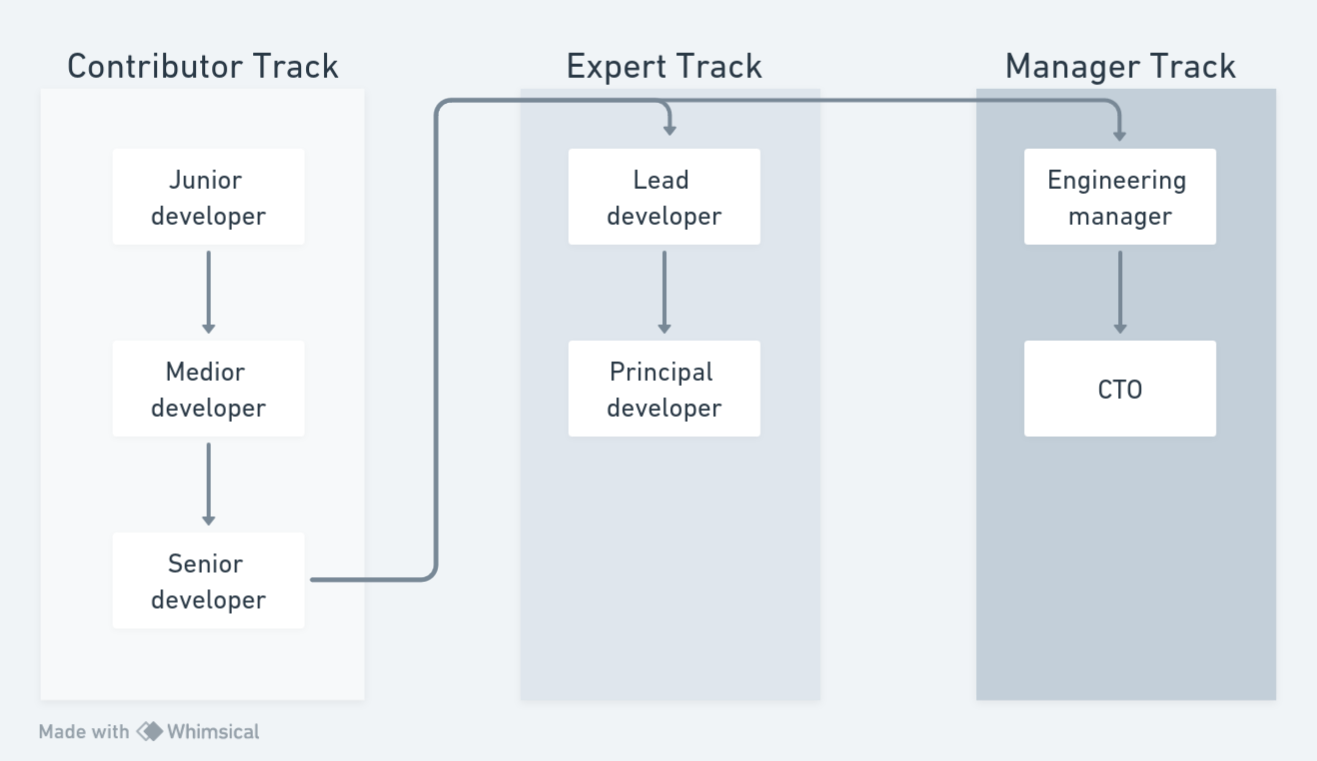
\includegraphics[width=\textwidth]{images/tracks.png}

\begin{multicols}{2}
  Pour un·e \dev, une carrière peut emprunter plusieurs chemins.
  Ces chemins ne sont pas rigoureusement étanches et des passages de l'un à l'autre sont possibles.

  \subsubsection*{Contributor Track}

  Dans tous les cas, une carrière commence avec la première position du premier parcours, nommé Contributor Track.
  Dans ce parcours, au travers des positions qui le composent, la personne acquiert des compétences clés pour être une
  excellente contributrice au projet.

  \subsubsection*{Expert Track}

  Après avoir atteint la position senior du Contributor Track, la personne peut choisir de se spécialiser 
  dans la technique, en choisissant le Expert Track.
  Si elle reste principalement contributrice, c'est un parcours qui l'amène sur le chemin de l'expertise technique.

  \subsubsection*{Manager Track}

  Après avoir atteint la position senior du Contributor Track, la personne peut choisir de se spécialiser 
  dans le management, en choisissant le Manager Track.
  C'est un parcours qui l'amène vers le management d'équipe et des individus qui la composent, pour les
  accompagner dans leur carrière et dans la réponse aux besoins de l'entreprise.

\end{multicols}

\part{Contributor Track}

\chapter{Junior developer}

Le junior developer est un professionnel récemment diplômé ou avec peu d’expérience. 
Il travaille sous la supervision d'autres développeurs plus expérimentés.

\xp{0 à 2}

\begin{multicols}{2}

  \paragraph{\dex{jd-01}} 

  Possède une connaissance approfondie des concepts fondamentaux de l'informatique.

  \paragraph{\dex{jd-02}} 

  Se concentre sur sa croissance en tant que \dev, en apprenant les outils, les ressources et les processus 
  existants.

  \paragraph{\str{jd-01}}

  Développe ses compétences en productivité en apprenant le contrôle de source, les éditeurs, le système de construction 
  et autres outils, ainsi que les meilleures pratiques de test.

  \paragraph{\str{jd-02}}

  Est capable de prendre des sous-tâches bien définies et de les accomplir.

  \paragraph{\wis{jd-01}}

  Développe ses connaissances sur un seul composant de l'architecture du projet.

  \paragraph{\cha{jd-01}}

  Est efficace dans la communication de l'état d'avancement à l'équipe et au management.

  \paragraph{\cha{jd-02}}

  Manifeste les valeurs fondamentales de l'entreprise, se concentre sur la compréhension et la mise en pratique de ces 
  valeurs.

  \paragraph{\cha{jd-03}}

  Accepte gracieusement les retours d'information constructifs et apprend de tout ce qu'iel fait.
\end{multicols}

\chapter{Medior developer}

Le medior developer possède une expérience solide et peut travailler de manière plus autonome.

\xp{2 à 5}

\begin{multicols}{2}

  \paragraph*{\dex{de-01}}

  Écrit du code fonctionnellement correct et propre avec des conseils ; suit systématiquement les meilleures pratiques 
  définies sur le projet.

  \paragraph*{\dex{de-02}}

  Participe à la conception technique des fonctionnalités avec des conseils.

  \paragraph*{\dex{de-03}}

  Fait rarement la même erreur deux fois, commence à se concentrer sur l'acquisition d'une expertise dans un ou plusieurs 
  domaines (par exemple : développement dans un langage donné, meilleures pratiques de performance, utilisation efficace 
  des bases de données, messagerie, etc.)

  \paragraph*{\dex{de-04}}

  Apprend rapidement et progresse régulièrement sans avoir besoin de commentaires significatifs constants de la part 
  de \devs\ plus expérimenté·es.

  \paragraph*{\str{de-01}}

  Fait des progrès réguliers sur les tâches ; sait quand demander de l'aide pour se débloquer.

  \paragraph*{\str{de-02}}

  Est capable de prendre en charge des fonctionnalités de petite à moyenne envergure, de la conception technique à 
  l'achèvement.

  \paragraph*{\str{de-03}}

  Est capable de hiérarchiser les tâches ; évite de s'enliser dans des détails sans importance et des "discussions sans 
  fin".

  \paragraph*{\wis{de-01}}

  Est autonome dans au moins un grand domaine du code avec une compréhension globale des autres composants.

  \paragraph*{\wis{de-02}}

  Est capable d'assurer une assistance en cas d'urgence pour leur domaine, y compris les systèmes avec lesquels iel 
  n'est pas familier·ère.

  \paragraph*{\cha{de-03}}

  Donne des commentaires opportuns et utiles aux pairs et au management.

  \paragraph*{\cha{de-04}}

  Communique les hypothèses et obtient des éclaircissements sur les tâches dès le départ afin de minimiser le besoin de 
  retravailler le code pendant la phase d'implémentation.

  \paragraph*{\cha{de-05}}

  Sollicite les commentaires des autres et est désireux de trouver des moyens de s'améliorer.

  \paragraph*{\cha{de-06}}

  Comprend comment son travail s'inscrit dans le projet global et identifie les problèmes liés aux exigences.

\end{multicols}

\chapter{Senior developer}

Le senior developer a une expertise approfondie et peut prendre en charge des projets complexes.

\xp{5 à 8}

\begin{multicols}{2}

  \paragraph*{\dex{sd-01}}

  Comprend et prend des décisions de conception bien raisonnées et des compromis dans son domaine.

  \paragraph*{\dex{sd-02}}

  Est capable de travailler dans d'autres domaines du code avec des conseils.

  \paragraph*{\dex{sd-03}}

  Garde son calme lors du débogage pour le mener à terme.

  \paragraph*{\dex{sd-04}}

  Démontre une connaissance des tendances de l'industrie, de l'infrastructure du projet et de son système de 
  construction.

  \paragraph*{\str{sd-01}}

  Estersistant face aux obstacles ; les résout efficacement, en faisant appel à d'autres personnes si nécessaire. 

  \paragraph*{\str{sd-02}}

  Nécessite un minimum de direction et de supervision.

  \paragraph*{\str{sd-03}}

  Prend l'initiative de résoudre les problèmes avant qu'ils ne lui soient assignés. 

  \paragraph*{\str{sd-04}}

  Livre des produits complexes à l'équipe de QA / Produit, qu'iel estime bien préparés et exempts de bugs.

  \paragraph*{\str{sd-05}}

  Recherche des preuves empiriques par le biais de preuves de concept, de tests et de recherches externes.

  \paragraph*{\wis{sd-01}}

  Est responsable de bout en bout sur des projets de complexité croissante ; contribue au code commun.

  \paragraph*{\wis{sd-02}}

  Examine les cas de test et conseille l'équipe de QA / Produit sur l'impact du code adjacent et les risques de 
  régression.

  \paragraph*{\wis{sd-03}}

  Comprend l'activité commerciale afférente à son domaine d'activité.

  \paragraph*{\wis{sd-01}}

  Collabore avec le produit et définit des exigences fonctionnelles et techniques 
  qui tiennent compte des besoins de toutes les parties.

  \paragraph*{\wis{sd-02}}

  Fait preuve d'empathie envers l'utilisateur du logiciel qu'iel produit et utilise cette empathie pour orienter la 
  prise de décision.

  \paragraph*{\wis{sd-03}}

  Identifie les problèmes et les risques dans son propre travail et dans celui des autres.

  \paragraph*{\cha{sd-01}}

  Communique les décisions techniques par le biais de documents de conception ou de présentations techniques.

  \paragraph*{\cha{sd-02}}

  Mentore les \devs\ juniors par le biais de la collaboration, de l'examen de conception et de l'examen de code. 

  \paragraph*{\cha{sd-03}}

  Communique efficacement entre les fonctions.
  Est capable de bien travailler avec le produit, le design, l'analyse, etc., si nécessaire.

  \paragraph*{\cha{sd-04}}

  Identifie de manière proactive les problèmes liés aux exigences (manque de clarté, incohérences, limitations 
  techniques) pour son propre travail et le travail adjacent, et communique ces problèmes tôt pour aider à corriger le 
  tir.

  \paragraph*{\cha{sd-05}}

  Contribue fréquemment aux réunions informelles et aux démonstrations.

\end{multicols}

\part{Expert Track}

\chapter{Lead developer}

Le lead developer est responsable de la coordination technique d'un ou plusieurs projets.

\xp{6 à 10}

\begin{multicols}{2}

  \paragraph*{\dex{ld-01}}

  Est l'expert de référence dans un domaine spécifique du code.

  \paragraph*{\dex{ld-02}}

  Comprend l'architecture globale de l'ensemble du système.

  \paragraph*{\dex{ld-03}}

  Fournit des conseils techniques et donne son avis sur les décisions techniques qui ont un impact sur d'autres équipes ou
  sur l'entreprise dans son ensemble. 

  \paragraph*{\dex{ld-04}}

  Effectue proactivement des recherches et propose de nouvelles technologies.

  \paragraph*{\str{ld-01}}

  Définit et organise le travail en étapes bien définies pour éviter un livrable monolithique.

  \paragraph*{\str{ld-02}}

  Livre régulièrement dans les délais et assure un travail constant pour faire des estimations précises et les 
  respecter.

  \paragraph*{\str{ld-03}}

  Est réputé pour des lancements sans problème.

  \paragraph*{\str{ld-04}}

  Est responsable du plan de tests techniques et du plan de performances pour ses projets.

  \paragraph*{\wis{ld-01}}

  Prend l'initiative d'identifier et de résoudre des problèmes importants, en se coordonnant avec d'autres personnes sur
  des problèmes techniques transversaux.

  \paragraph*{\wis{ld-02}}

  Définit l'orientation au niveau du projet et influence de manière constante la prise de décision au niveau
  technique.
  \paragraph*{\wis{ld-03}}

  Identifie et aborde de manière proactive la dette technique avant qu'elle ne devienne trop coûteuse à rembourser.

  \paragraph*{\cha{ld-01}}

  Aide les autres personnes à s'améliorer grâce à des revues de code, une documentation approfondie, des conseils 
  techniques et un mentorat ou en tant que chef technique sur un projet.

  \paragraph*{\cha{ld-02}}

  Siège aux comités de prise de décisions techniques ou architecturales, et donne des commentaires sur des projets en 
  dehors de son domaine principal.
  
  \paragraph*{\cha{ld-03}}

  Comprend les compromis entre les besoins techniques, analytiques et produits et propose des solutions qui tiennent 
  compte de tous ces besoins.

  \paragraph*{\cha{ld-04}}

  Identifie et propose des stratégies pour résoudre les problèmes techniques affectant son équipe, communique des normes 
  et obtient l'adhésion aux solutions.

\end{multicols}

\chapter{Principal developer}

Le principal developer est un expert technique qui influence la stratégie de développement.

\xp{10 à 15}

\begin{multicols}{2}

  \paragraph*{\dex{pd-01}}

  Est sollicité pour des conseils techniques.
  
  \paragraph*{\dex{pd-02}}

  Anticipe les problèmes techniques au niveau du produit et prend des décisions architecturales et de conception pour les 
  éviter.

  \paragraph*{\dex{pd-03}}

  Est propriétaire et expert de grandes parties de la base de code.
  
  \paragraph*{\dex{pd-04}}

  A accumulé un historique d'améliorations majeures en termes de stabilité, de performance et de scalabilité sur des 
  systèmes critiques pour l'entreprise.

  \paragraph*{\str{pd-01}}

  Est reconnu comme un contributeur prolifique aux projets principaux et aux projets annexes.

  \paragraph*{\str{pd-02}}

  Est capable de réduire systématiquement la complexité des projets, des services et des processus afin de faire plus 
  avec moins de travail.

  \paragraph*{\wis{pd-01}}

  Définit l'architecture globale.

  \paragraph*{\wis{pd-02}}

  Déploie plusieurs services importants, des bibliothèques complexes ou des éléments d'infrastructure majeurs.

  \paragraph*{\wis{pd-03}}

  A eu un impact positif évident sur la trajectoire technique de l'ensemble de l'entreprise.

  \paragraph*{\cha{pd-01}}

  Multiplie l'efficacité des autres en facilitant le travail inter-équipes.

  \paragraph*{\cha{pd-02}}

  Écoute et guide les débats pour aider à parvenir à un consensus.
  Une fois une décision prise, communique clairement et soutient cette décision.

  \paragraph*{\cha{pd-03}}

  Définit la direction technique stratégique à court et moyen terme.
  Est capable de prévoir les besoins les plus importants  sur 6 à 12 mois et de créer des plans d'amélioration.

  \paragraph*{\cha{pd-04}}

  Communique l'excellence technologique de l'entreprise à l'extérieur via des conférences et des articles de blog. 
  
  \paragraph*{\cha{pd-05}}

  Identifie les domaines que l'entreprise peut partager efficacement avec le monde extérieur et guide la création de 
  contenu et de communication autour de ces domaines.

  \paragraph*{\cha{pd-06}}

  Mène les discussions internes sur l'orientation des principaux domaines de la technologie, favorise un consensus élargi
  pour l'adoption de cette orientation et utilise cette orientation pour inspirer les équipes techniques.
  
  \paragraph*{\cha{pd-07}}

  Est considéré comme un modèle et un mentor pour chaque membre de l'équipe technique.

\end{multicols}

\part{Manager Track}

\chapter{Engineering manager}

L'engineering manager supervise et accompagne les équipes de développement.

\begin{multicols}{2}

  \paragraph*{\dex{em-01}}

  Comprend et pratique le développement et la gestion agile de logiciels.

  \paragraph*{\dex{em-02}}

  Produit des métriques de qualité sur le processus de développement du cycle de vie des logiciels.
  
  \paragraph*{\dex{em-03}}

  Veille à ce que les logiciels soient surveillables et hautement disponibles.

  \paragraph*{\str{em-01}}

  Progresse en déléguant efficacement.
  
  \paragraph*{\str{em-02}}

  Veille à ce que les tâches soient réalisées conformément aux spécifications, mais sans microgestion.

  \paragraph*{\str{em-03}}

  Est proactif dans l'identification et l'élimination des obstacles pour l'équipe.

  \paragraph*{\str{em-04}}

  Continue à contribuer à la correction des bogues et aux fonctionnalités sans devenir un goulet d'étranglement pour 
  l'équipe.

  \paragraph*{\wis{em-01}}

  Est axé sur la productivité de l'équipe et son impact collectif.

  \paragraph*{\wis{em-02}}

  Amène l'équipe à se concentrer sur les projets les plus impactants.

  \paragraph*{\wis{em-03}}

  Est capable de diriger les efforts de recrutement et de déterminer les effectifs pour son équipe.
  
  \paragraph*{\wis{em-04}}

  Collabore efficacement avec le produit pour gérer la portée et les livrables de la feuille de route technique du 
  produit.

  \paragraph*{\cha{em-01}}

  Prend des décisions pour les besoins de l'équipe.
  
  \paragraph*{\cha{em-02}}

  Apprend activement à gérer des situations de management difficiles.

  \paragraph*{\cha{em-03}}
  
  Contribue au développement de carrière des autres.
  
  \paragraph*{\cha{em-04}}

  Se réunit régulièrement avec ses collaborateurs directs, fournit des commentaires fréquents sur leur travail, aide les
  individus à fixer des objectifs et travaille avec le top management pour garantir la  croissance et la rétention des 
  employés.

  \paragraph*{\cha{em-05}}

  Gère de manière indépendante.
  
  \paragraph*{\cha{em-06}}

  Communique le contexte à l'équipe et expose les exigences à la direction.

  \paragraph*{\cha{em-07}}

  Définit des attentes claires pour les membres de l'équipe.
  
  \paragraph*{\cha{em-08}}

  Sollicite, synthétise et fournit des commentaires.
  
  \paragraph*{\cha{em-09}}

  Communique les délais, la portée et les préoccupations techniques aux parties prenantes.
  
  \paragraph*{\cha{em-10}}

  Dirige la réalisation des principales initiatives dans des délais clairs.
  
  \paragraph*{\cha{em-11}}

  Est capable d'identifier les domaines de la dette technique stratégique et de fournir une analyse coûts/avantages pour 
  éliminer cette dette.
  Propose des échéanciers pour le faire.
  
  \paragraph*{\cha{em-12}}

  Est capable de gérer des membres d'équipe ayant des compétences et des domaines techniques différents.

\end{multicols}

\chapter{CTO}

Le CTO est responsable de la stratégie technologique de l’entreprise.

\begin{multicols}{2}

  \paragraph*{\dex{ct-01}}

  Définit la direction technique de l'entreprise.

  \paragraph*{\dex{ct-02}}

  Définit les priorités organisationnelles de l'ingénierie.

  \paragraph*{\dex{ct-03}}

  Veille à ce que l'architecture en cours de construction puisse prendre en charge plusieurs possibilités futures de 
  l'entreprise.

  \paragraph*{\str{ct-01}}

  Met l'accent sur la réalisation des objectifs.

  \paragraph*{\wis{ct-01}}

  Est capable d'identifier les opportunités de croissance commerciale offertes par la technologie et de les concrétiser.

  \paragraph*{\cha{ct-01}}

  Communique la stratégie au niveau de la direction et contribue à traduire les directives commerciales en objectifs 
  technologiques.

\end{multicols}

\backmatter

\chapter*{Fiche de carrière}

\todo{fiche}

\chapter*{À propos}

\begin{multicols}{2}
  \section*{Source}
  
  Ce référentiel est issue du post de blog 
  "Sharing Our Engineering Ladder"\footnote{\url{https://dresscode.renttherunway.com/blog/ladder}}
  de la société Rent the Runway.
  
  Il a ensuite été traduit et retravaillé.
  
  \section*{Images}
  
  Photo de couverture par Annie Spratt\footnote{\url{https://unsplash.com/fr/@anniespratt}} sur Unsplash.
  
  \section*{Propriété intellectuelle}
  
  Ce document constitue une \oe uvre originale, protégée par le droit d'auteur tel que défini par le droit français.
  Toute reproduction, diffusion, publication ou retransmission de son contenu est strictement interdite sans 
  l'autorisation écrite du détenteur des droits d'auteur.
\end{multicols}

\tableofcontents

\end{document}
